% --------------------------------------------------------------
%                           Set Up
% --------------------------------------------------------------
 
\documentclass[12pt]{article}
 
\usepackage[margin=1in]{geometry} 
\usepackage{amsmath,amsthm,amssymb}
\usepackage{listings}
\usepackage{xcolor}
\usepackage{graphicx}
\usepackage{subcaption}
\usepackage{listings}
\usepackage{xcolor}
\usepackage{comment}
\usepackage{hepnames}
 
\definecolor{codegreen}{rgb}{0,0.6,0}
\definecolor{codegray}{rgb}{0.5,0.5,0.5}
\definecolor{codepurple}{rgb}{0.58,0,0.82}
\definecolor{backcolour}{rgb}{0.95,0.95,0.92}
 
\lstdefinestyle{mystyle}{
    backgroundcolor=\color{backcolour},   
    commentstyle=\color{codegreen},
    keywordstyle=\color{magenta},
    numberstyle=\tiny\color{codegray},
    stringstyle=\color{codepurple},
    basicstyle=\ttfamily\footnotesize,
    breakatwhitespace=false,         
    breaklines=true,                 
    captionpos=b,                    
    keepspaces=true,                 
    numbers=left,                    
    numbersep=5pt,                  
    showspaces=false,                
    showstringspaces=false,
    showtabs=false,                  
    tabsize=2
}
 
\lstset{style=mystyle}
 
\definecolor{codegreen}{rgb}{0,0.6,0}
\definecolor{codegray}{rgb}{0.5,0.5,0.5}
\definecolor{codepurple}{rgb}{0.58,0,0.82}
\definecolor{backcolour}{rgb}{0.95,0.95,0.92}
\definecolor{deepblue}{rgb}{0,0,0.5}
\definecolor{deepred}{rgb}{0.6,0,0}
\definecolor{deepgreen}{rgb}{0,0.5,0}
 
\lstdefinestyle{mystyle}{
    backgroundcolor=\color{backcolour},   
    commentstyle=\color{codegreen},
    keywordstyle=\color{deepred},
    numberstyle=\tiny\color{codegray},
    stringstyle=\color{deepblue},
    basicstyle=\ttfamily\footnotesize,
    breakatwhitespace=false,         
    breaklines=true,                 
    captionpos=b,                    
    keepspaces=true,                 
    numbers=left,                    
    numbersep=5pt,                  
    showspaces=false,                
    showstringspaces=false,
    showtabs=false,                  
    tabsize=2
}
 
\lstset{style=mystyle}
 
\newcommand{\N}{\mathbb{N}}
\newcommand{\Z}{\mathbb{Z}}
 
\newenvironment{theorem}[2][Theorem]{\begin{trivlist}
\item[\hskip \labelsep {\bfseries #1}\hskip \labelsep {\bfseries #2.}]}{\end{trivlist}}
\newenvironment{lemma}[2][Lemma]{\begin{trivlist}
\item[\hskip \labelsep {\bfseries #1}\hskip \labelsep {\bfseries #2.}]}{\end{trivlist}}
\newenvironment{exercise}[2][Exercise]{\begin{trivlist}
\item[\hskip \labelsep {\bfseries #1}\hskip \labelsep {\bfseries #2.}]}{\end{trivlist}}
\newenvironment{problem}[2][Problem]{\begin{trivlist}
\item[\hskip \labelsep {\bfseries #1}\hskip \labelsep {\bfseries #2.}]}{\end{trivlist}}
\newenvironment{question}[2][Question]{\begin{trivlist}
\item[\hskip \labelsep {\bfseries #1}\hskip \labelsep {\bfseries #2.}]}{\end{trivlist}}
\newenvironment{corollary}[2][Corollary]{\begin{trivlist}
\item[\hskip \labelsep {\bfseries #1}\hskip \labelsep {\bfseries #2.}]}{\end{trivlist}}

\newenvironment{solution}{\begin{proof}[Solution]}{\end{proof}}

\setlength\parindent{0pt}
 
\begin{document}
 
% -------------------------------------------------------------- 
%                         Start here
% --------------------------------------------------------------
 
\title{Homework 4}
\author{Timothy Holmes\\ %replace with your name
PHY 475 Introduction to Cosmology}

\maketitle

\section*{Problem 7.3}
The equation to find the angle of deflected light by a massive object is found in equation 7.43. The angle $\alpha$ is given as

$$
\alpha = \frac{4GM}{c^{2}b}
$$

where $b$ is the mass of the massive object, $c$ is the speed of light, $M$ is the mass is the massive object, and $G$ is the gravitational constant. Therefore, the light that grazes the Earths surface is deflected at an angle of 

$$
\alpha = \frac{4*6.7*10^{-11}m^{3}kg^{-1}s^{-2}*6.0*10^{24}kg}{(3.0*10^{8}ms^{-1})^{2}*6.4*10^{6}m} = \boxed{2.8*10^{-9} rad}.
$$

The light that grazes a white dwarf surface with mass $M = 2.0*10^{24} kg$ and radius $R = 1.5*10^{7} m$ is deflected at an angle of 

$$
\alpha = \frac{4*6.7*10^{-11}m^{3}kg^{-1}s^{-2}*2.0*10^{24}kg}{(3.0*10^{8}ms^{-1})^{2}*1.5*10^{7}m} = \boxed{4.0*10^{-4} rad}.
$$

Finally, the light that grazes a neutron star surface with mass $M = 3.0*10^{24} kg$ and radius $R = 1.2*10^{4} m$ is deflected at an angle of 

$$
\alpha = \frac{4*6.7*10^{-11}m^{3}kg^{-1}s^{-2}*3.0*10^{24}kg}{(3.0*10^{8}ms^{-1})^{2}*1.2*10^{4}m} = \boxed{7.4*10^{-1} rad}.
$$

From the results above we see that objects with the largest mass and smallest radius deflect the light at greater angles. Intuitively, this should make sense since these objects have more of a profound effect on the spacetime fabric. This can also be seen in the equation, if the mass is large the numerator is larger and if the radius is small the denominator is smaller. Based of the equation, it shows that objects as such will result in having more of an affect on light.

\section*{Problem 7.4}

The density of an object can be found by knowing the objects mass and volume. Density is found by

$$
\rho = \frac{M}{V}
$$

where $M$ is mass and $V$ is volume. Equation 7.31 says that the mass of a self-gravitating steady-state system is 

$$
M = \frac{\langle v^2 \rangle r_{h}}{\alpha G}.
$$

The halo has a volume of $4\pir^{2}dr$ with density $4\pir^{2}dr \rho$. The mass of the halo is then $dM = 4\pir^{2}dr \rho$. Differentiating and solving for $\rho$ yields 

$$
\rho = \frac{\langle v^2 \rangle}{\alpha G 4\pi r^{2}}
$$

At $\Omega_{Lambda, 0} = 0.7$ the universe is Dark Matter dominated. Looking at the galaxy rotation curve this scenario would be affected the dynamics of the galaxy's halo.

last part no, it will not affect much


\iffalse
\section*{Problem 7.6}

The fusion reaction in the Sun's core produces

$$
2*10^{38} \Pneutrino/s
$$

Assuming that we are a sphere shaped then the surface area of a human liked object is needed. A human is $~1m$ give or take $0.5m$. The surface area of a sphere is as follows $A = 4\pi r^2$. If our human is $1m$ in height then the radius of that human with the assumption of a sphere is $0.5m$. The surface area of our human becomes $A = 4\pi (0.5m)^2 = 3.141m^2$. To find the frequency of solar neutrinos that hits the human surface is found using 

$$
n_{\gamma}*c*A = 2*10^{38} \Pneutrino/s*3.00*10^{8}m*s^{-1}*3.14m^{2} = 3.87*10^{17} s^{-1}
$$
\fi

\section*{Problem 3}

The equation of state equation is gave by

$$
P = w*\epsilon.
$$

This gives the equation of state as $P = -\epsilon$ showing $w = -1$ which means that this universe is a single component matter dominated universe. If the scale factor were to increase by 60 e-foldings, the new $\Omega$ would start from equation 10.27,

$$
|1 - \Omega(t_{f})| = e^{-2N}|1 - \Omega(t_{i})|.
$$

Entering in the initial $Omega$ and N gives

$$
|1 - \Omega(t_{f})| = e^{-2*60}|1 - 0.5| \ \rightarrow |1 - \Omega(t_{f})| = e^{-120} 0.5.
$$

Therefore,

$$
\Omega(t_f) \approx 1.
$$

The initial omega value has no affect on the exponential since it will always dominate as long as $N$ is greater than 1. $\Omega$ is still 1 the universe would still be flat at $T = 10^{4} K$.



\section*{Problem 11.4}

Starting with equation 11.3 from the text the average density is $\bar{\rho} = 3M/(4\pi R_{halo}^{3})$. Therefore, $t_{min}$ becomes

$$
t_{min} \approx \frac{1}{\sqrt{G\bar{\rho}}} = \sqrt{\frac{4\piR_{halo}^{3}}{3GM}}.
$$

The rotation speed $v$ for a disk galaxy is given by the virial theorem in equation 7.10. Solving for mass equation 7.10 becomes $M = v^{2}R_{halo}/G$. Entering mass given by the virial theorem into the equation above yields 

$$
\sqrt{\frac{4\pi R_{halo}^{3}G}{Gv^{2}R_{halo}G}} = \sqrt{\frac{4\pi R_{halo}^{2}}{v^{2}}}
$$.

Which is approximately 

$$
t_{min} \approx \sqrt{4\pi}\frac{R_{halo}}{v}.
$$

For our galaxy $R = 75 kpc$ and $v = 235 km s^{-1}$. Thus,

$$
t_{min} = 300*10^{6} yr.
$$

From equation 11.58 we find that

$$
t^{2/3} \propto a(t) \propto \frac{1}{1 + z}.
$$

Then, equation 5.112 shows 

$$
a = (3/2\sqrt{\Omega_{m,0}}H_{0}t)^{2/3}
$$

From the equation above we can solve for z as 

$$
z = (3/2\sqrt{\Omega_{m,0}}H_{0}t)^{-2/3} - 1
$$

and find that $z = 13$.

\section*{Problem 5}

\begin{figure}[h!]
    \centering
    \subfloat[Figure 1]{{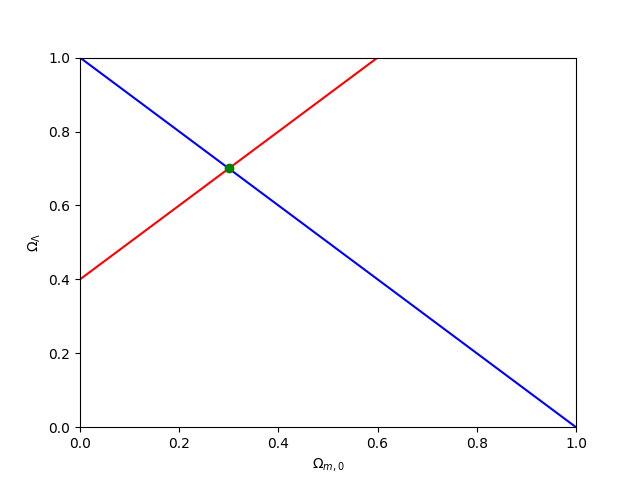
\includegraphics[width=14cm]{figure1.png}}}%
    \qquad
    \caption{Problem 5}%
    \label{fig:example}%
\end{figure}

The intersection, where the green dot is, is the current day values for $\Omega_{m,0} = 0.3$ and $\Omega_{\Lambda,0} = 0.7$. The Friedmann equation is given by 

$$
\Big(\frac{\dot{a}}{a}\Big) = \frac{\Omega_{r}}{a^{4}} + \frac{\Omega_{m}}{a^3} + \Omega_{\Lambda}. 
$$

If $a = 0$ in the present time then the equation becomes $\Omega_{m} - \Omega_{\Lambda} = 0.4$ which means the acceleration is positive and for the equation to be positive, $\Omega_{m} > \Omega_{\Lambda}$ which means its matter dominated. This changes the benchmark model and when the big bang/crunch occurs. 

\section*{Appendix}

\begin{lstlisting}[language=Python, caption= Problem 8.2 plotting code]
import numpy as np
import matplotlib.pyplot as plt


#--------- initial conditions ----------
omega_m = np.array( np.linspace(0, 1.0, 100))
omega_lambda = 1 - omega_m
plt.plot(omega_m, omega_lambda, 'b-')


omega_lambda = omega_m + 0.4
plt.plot(omega_m, omega_lambda, 'r-')


#--------- omega values ----------
benchmark_omega_m = 0.3
benchmark_omega_lambda = 0.7

plt.plot(benchmark_omega_m, benchmark_omega_lambda, 'go')
plt.xlabel(r"$\Omega_{m, 0}$")
plt.ylabel(r"$\Omega_{\Lambda}$")
plt.xlim(0, 1)
plt.ylim(0, 1)
plt.savefig('./figure1.png')
plt.show()
\end{lstlisting}


% --------------------------------------------------------------
%                           End Document.
% --------------------------------------------------------------
 
\end{document}

